
\title{Recap Database Management System (01NVVOV)}
\author{Jacopo Nasi\\
        Computer Engineer\\
        Politecnico di Torino}
\date{I Period - 2017/2018\\\bigskip\bigskip\today}

\documentclass[12pt]{article}
\usepackage[utf8]{inputenc}
\usepackage[italian]{babel}
\usepackage{geometry}
\usepackage{indentfirst} % First line indent
\usepackage{mathtools}
\usepackage{wrapfig}
\usepackage[usenames, dvipsnames]{color}
\usepackage{float}
\usepackage{amssymb}
\usepackage{ifsym}
% Misure Documento
\geometry{ a4paper, total={170mm,257mm},left=35mm, right=35mm, top=35mm, bottom=35mm }

\begin{document}

\begin{figure}
  \centering
  
\includegraphics[width=10cm]{images/polito.pdf}
\end{figure}

\maketitle

\newpage
\tableofcontents

\newpage
{\noindent \Large \textbf{License}\bigskip}

This work is licensed under a Creative Commons Attribution-NonCommercial-ShareAlike 3.0 Unported License.\\
You are free:
\begin{itemize}
  \item \textbf{to Share}: to copy, distribute and transmit the work
  \item \textbf{to Remix}: to adapt the work
\end{itemize}
Under the following conditions:
\begin{itemize}
  \item \textbf{Attribution}: you must attribute the work in the manner specified by the author or licensor (but not in any way that suggests that they endorse you or your use of the work)
  \item \textbf{Noncommercial}: you may not use this work for commercial purposes.
  \item \textbf{Share Alike}: if you alter, transform, or build upon this work, you may distribute the resulting work only under the same or similar license to this one.
\end{itemize}

\noindent More information on the Creative Commons website (http://creativecommons.org).

\begin{figure}[h!]
  \centering
  
\includegraphics[width=3cm]{images/license.png}
\end{figure}

{\noindent \Large \textbf{Acknowledgments}\bigskip}

Questo breve riepilogo non ha alcuno scopo se non quello di agevolare lo studio di me stesso, se vi fosse di aiuto siete liberi di usarlo.\\
Le fonti su cui mi sono basato sono quelle relative al corso offerto (\textbf{Database Management System (01NVVOV)}) dal Politecnico di Torino durante l'anno accademico 2017/2018.\\
Non mi assumo nessuna responsabilità in merito ad errori o qualsiasi altra cosa. Fatene buon uso!
\newpage

\section{Database Management System}
\subsection{Introduction}

The DataBase Management System \textbf{DBMS} is a software package designed to store and manage databases. The architecture of the system is similar to the one in the figure \ref{fig:arch}.
\begin{figure}[h!]
  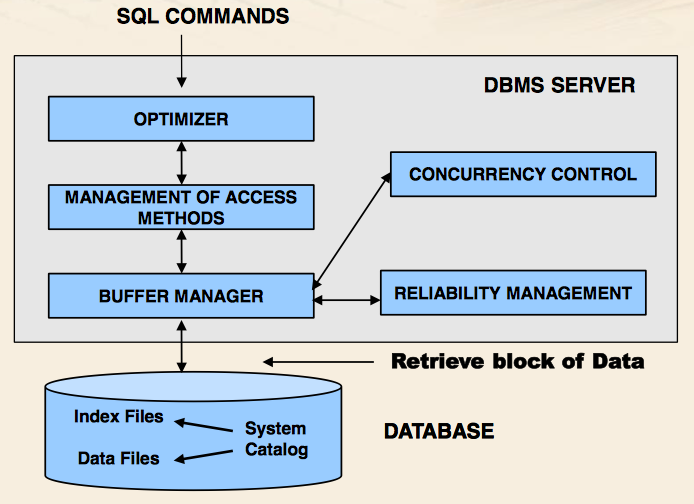
\includegraphics[width=\linewidth]{images/arch.png}
  \caption{DBMS Architecture}
  \label{fig:arch}
\end{figure}
Since the DB data part can be really big it can't fit always in the main memory (RAM) and, for this fact, is often stored in the secondary memory, like HDD. For this reason is necessary a system that define the operations to grab and manage the data from the secondary memory.\\
All the blocks has different behaviours. The \textbf{Optimizer} have multiple roles:
\begin{itemize}
  \item Define an appropriate execution strategy for accessing data to answer queries.
  \item Receives in input the SQL instructions (DML).
  \item Check the lexical, syntactical and sematical correctness (not all the errors).
  \item Translate the query in an internal algebra rappresentation.
  \item Select the "right" strategy for accesing data.
  \item Guarantees the \textbf{data independence} property in the relation model.
\end{itemize}
The \textbf{Access Method Manager} is used for physical access to data and it implements the strategy selected by the optimizer. The \textbf{Buffer Manager} instead manage the page transfert from disk to main memory and vice versa and the main memory portion that is pre-allocated to the DBMS that is shared among many applications. The \textbf{Concurrency Control} coordinate the concurrent access to data (important for write operations) to guarantess the consistency of it. The \textbf{Realiability Manager} guarantees correctness of the database content duing the system crashes, the atomic execution of a transaction and it exploits auxiliary structures (log files) the correct the database in case of failure.\\
The \textbf{transaction} is an unit of work performed by an application, it's a sequence of one or more SQL RW operation charaterized by \textit{correctness, reliability} and \textit{isolation}. The START of a transaction is typically implicit and coincides with the first SQL instruction. The END instead can be of two differents types, it can be a COMMIT that it means the correct end of a transaction, or with ROLLBACK that it means error during the execution. In this second case the DBMS needs to go back to the state at the beginning of the transaction. The rollback can be of two type suicide, when is required by the transaction, and murder when is required by the system. The transaction have four important properties:
\begin{itemize}
  \item \textbf{A}tomicity
  \item \textbf{C}onsistency
  \item \textbf{I}solation
  \item \textbf{D}urability
\end{itemize}
Atomicity means that they cannot be divided in smaller units, is not possibile to leave the system in a intermediate state of exec, guarantee by UNDO (undoes all the work perfomed, used for rollback) and REDO (redoes all work performed, used for commit the result in presence of failure). The consistency means that the transaction execution should not violate integrity constraints on a database, in case of it the system will perform solution to correct the violation. The system can be considered Isolated when the execution of a transaction is indipendent of the concurrent execution of other transaction, everything is enforced by the Concurrency Control block. The last properties means that, in presence of failures, the effect of a commited transaction IS NOT LOST, it guarantees the reliability of the DBMS and is enforced by the Reliability Manager block. % 3/9/17 @ 18:15

\subsection{Buffer Manager}
This block have a real important behaviour, it manages page transfer from disk to main memory and it's in charge of managing the DBMS buffer. The operation of the pages trasnfert is the bottleneck of every system and this is why this block is really important. increasing the performance of this operation could really improve the speed of the entire system.\\
The buffer is:
\begin{itemize}
  \item A large main memory block.
  \item Pre-allocated to the DBMS.
  \item Shared among executing transactions.
\end{itemize}
this part is organized in pages where the size depends on the size of the OS I/O block. There are two empirical law often used for hte management strategies:
\begin{enumerate}
  \item Data Locality: Data referenced recntly is likely to be referenced again.
  \item 20-80: The 20\% of data is RW by 80\% of transaction.
\end{enumerate}
The buffer manager keeps additional snapshot information on the current content of the buffer, it shot, for every page, the physical location of the page on the secondary memory (file identifier and block number) and two state variables, one that count of the number of trasn using the page in that time (count), and the dirty bit that is set if the page has been modified.\\ %Set No. 2 @ PAG. 8
It provides different access methods to load pages from disk and vice versa:
\paragraph{Fix Primitive} used by transactions to require access to a disk page, after the page is loaded into the buffer a pointer is returned to the requesting transaction and the Count is incremented by 1. This procedure requires an I/O operation only id the page is not already in the buffer. There are two behaviour:
\begin{itemize}
  \item Page already in buffer: Return the pointer to the data.
  \item Page not in buffer: It search a place for the page.
  \begin{enumerate}
    \item Free pages
    \item Not free pages, Count=0; if the data is dirty it performs a synchronous write on the disk.
  \end{enumerate}
\end{itemize}
\paragraph{Unfix Primitive} it tells the buffer manager that the transaction is no longer using the page and it decrease the Count.
\paragraph{Set Dirty Primitive} is tells the buffer manager that the page has been modified by the running transaction and it sets the dirty bit to 1.
\paragraph{Force Primitive} it requires a synchronous transfert of the page to the disk, when this operation is performed the transaction is suspended.
\paragraph{Flush Primitive} is an autonomous transfert of the pages on the disks, is internal to the buffer manager and is runned when the CPU is not too much loaded. It transfer the page that are not valid (count=0) or not accessed since long time.\\
The are four writing strategies:
\begin{itemize}
  \item \textbf{Steal}: The BM is allowed to select a locked page with Count=0 as victim. It writes on disk the dirty pages belonging to uncommitted trans. It can be undone.
  \item \textbf{No Steal}: The BM is not allow to steal.
  \item \textbf{Force}: All the pages are synchronous written on the disk during the commit operation.
  \item \textbf{No Force}: The pages are written asynchronously with the Flush Primitive.
\end{itemize}
The mostly used solution is \textbf{steal/no force} because of its efficency. The no force provides better I/O performance, steal may be mandatory for queries accessing a very large number of pages.

\paragraph{File System} the BM is using services provided by the file system:
\begin{itemize}
  \item Create/Delete of a file.
  \item Open/Close file.
  \item Read: It provides a direct access to a block in a file and it requires File Identifier, Block number and buffer page where to save data.
  \item Sequential Read: It provides seq. access to a fixed number of blocks in a file, it requires file identifier, strating block, number of blocks to be readed and the starting page for saving.
  \item Write and Sequential Write.
  \item Directory management.
\end{itemize} % END Block 2 - Buffer Manager

\subsection{Physical Access}
Data may be stored in different format to provide efficient query execution. The \textbf{Access Method Manager} transform the decision taken by the optimizer into sequence of physical access to data. An access method is a software module specialized for single data structure that provide primitives for read and write. The AM can select the appropriate blocks of a file to be loaded in memory and it knows the organization of data into a page.\\
There are several solution for manage the data in relational system:
\begin{itemize}
  \item Physical data storage
  \begin{itemize}
    \item Sequential Structure
    \item Hash Structure
  \end{itemize}
  \item Indexing
  \begin{itemize}
    \item Tree Structure
    \item Unclustered Hash Index
    \item Bitmap Index
  \end{itemize}
\end{itemize}

In the sequential solution the tuples are stored in a given sequential order, in the case of the heap file are sorted in the insertion order, typically append at the end of the file.
\begin{itemize}
  \item \textbf{PRO}: No wasted space, sequential read/write fast.
  \item \textbf{CONS}: Delete may cause wasted space.
\end{itemize}
this structure are frequently used jointly with unclustered indices to support search and sort operations.\\
In the ordered structures everything is sorted by the value of a given key, called sort key, it can contain one or more attributes.
\begin{itemize}
  \item \textbf{PRO}: Sort, group by, search or join operations on the sort key really fast.
  \item \textbf{CONS}: Inserting new value preserving order.
\end{itemize}
the main problem of this solution is to keep the order of the data during new data insertion. There are two main solution, the first il leaving a percentage of free space in each block during the table creation.

\bibliographystyle{abbrv}
\bibliography{simple}

\end{document}
